\begin{apendicesenv}
  
  \chapter{Processo de Engenharia de Requisitos}
  
    \begin{figure}[!htbp]
      \centering
      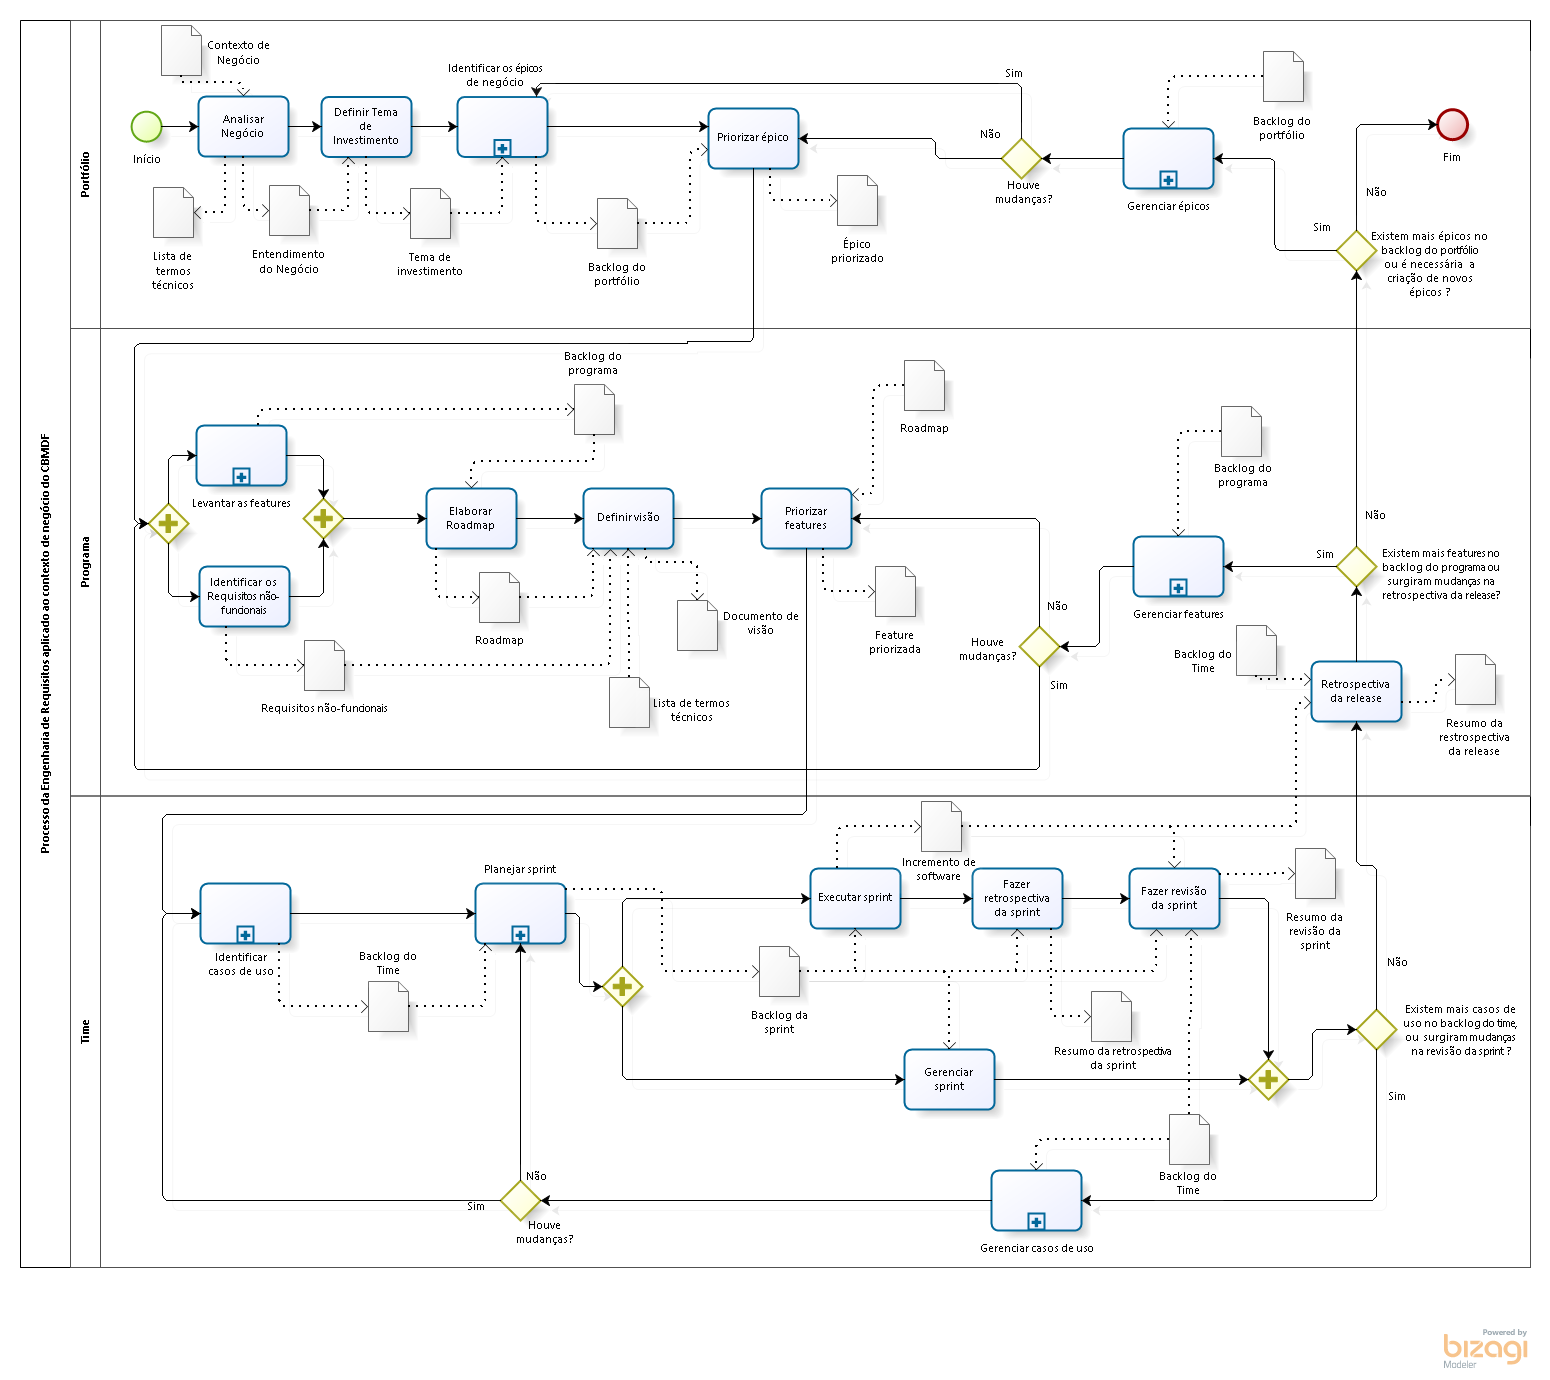
\includegraphics[scale=0.46, angle = 90]{editaveis/figuras/project_big_picture}
      \caption[Modelo do processo de Engenharia de Requisitos]
	  {Modelo do processo de Engenharia de Requisitos: \textit{Big Picture} do projeto.}
      \label{project_big_picture}
    \end{figure}
  
  \chapter{Documento de visão}
	{\centering
	\textbf{Corpo de Bombeiros Militar do Distrito Federal}

	\textbf{Documento de visão para o sistema de gerenciamento de viaturas}

	\textbf{2015}

	}
	\textbf{Histórico de Revisões}
	\begin{table}[h]
	\centering
	\label{my-label}
	\begin{tabular}{|l|l|l|l|}
	\hline
	Data & Revisão & Descrição & Autor \\ \hline
	14/06/2015 & 1.0 & Versão Inicial & João Paulo \\ \hline
	     &         &           &       \\ \hline
	     &         &           &       \\ \hline
	\end{tabular}
	\caption{Histórico de Revisões}
	\end{table}
  
	\section{Introdução}
		\subsection{Propósito}
Este documento define estratégias pretendidas para o programa. Isto define as principais necessidades do usuário qualquer interação pessoal com o produto, principais Stakeholder e o conjunto de capacidades gerais que o usuário necessita.
		\subsection{Resumo da solução}
Afirma a proposta geral dos produtos, sistema, Aplicação ou serviço e qualquer versão de identificação.
		•Identidade do produto ou aplicação para ser criado ou aperfeiçoamento
		•Descreve a aplicação do produto, incluindo os benefícios e objetivos
		•Providencia uma descrição geral de onde vai terminar e” where appropriate will not do.
		\subsection{Referências}
		Listar outros documentos de referência e especificar as fontes a partir das quais as referências podem ser obtidas. if business case( chapter 23) was developed to drive the program, refer to it or attach it.
	\section{Descrição do Usuário}
Lista de outros produtos e serviços que atendam as necessidades dos utilizadores, é útil para compreender os desafios que enfrentam ao realizar seus trabalhos. Esta seção deve perfilar os usuários do proposto para o  aplicativo e os principais problemas que limitam a produtividade do usuário. Esta seção não deve ser usado requisitos específicos de cada Estado; apenas fornecer o back-ground para o que o especificado no ponto 5 seja necessários.

		\subsection{Demografia de Usuário/Mercado}
Resume as principais demografias do mercado que motivam as decisões de solução. Descreva segmentos de mercado-alvo. Estima o tamanho do mercado e crescimento do número de usuários potenciais ou a quantidade de dinheiro que seus clientes gastam, tentando satisfazer a necessidade que o seu produto / realce iria cumprir. Revisão das principais tendências e tecnologias do setor que referem-se a uma análise de mercado, quando disponível.

		\subsection{\textit{User Personas}}
A
		\subsection{Ambiente de Usuário}
A
		\subsection{Principais necessidades do Usuários}
A
	
	\section{\textit{Stakeholders}}
A
		
	\section{Resumo do Produto}
A
		\subsection{Perspectiva do Produto}
A
		\subsection{Intenção do Produto}
A
		\subsection{Resumo das Capacidades}
A
		\subsection{Suposições e Dependências}
A
		\subsection{Preços e Custos}
A
	\section{\textit{Features} do Produto}
A
		\subsection{Feature 1}
A
		\subsection{Feature 2}
A
		\subsection{Feature 3}
A

	\section{Exemplos de Caso de uso}
A
	\section{Requisitos não-funcionais}		
A
		\subsection{RNF 1}
A
		\subsection{RNF 2}
A
		\subsection{RNF 3}
A
			\subsubsection{Padrões de aplicação}
A
			\subsubsection{Licença, segurança e aplicação}
A

	\section{Documentação dos Requisitos}
A
		\subsection{Manual do Usuário}
A
		\subsection{Ajuda Online}
A
		\subsection{Guia de instalação, configuração e arquivo \textit{ReadMe}}
A
		\subsection{Rotulagem dos requisitos e Empacotamentos}
A
		\subsection{Glossário}
A


\end{apendicesenv}
